\documentclass[11pt, letterpaper, twoside, final]{article}
\usepackage{risk_price_inference}
\addbibresource{riskpriceinference.bib}

\author{Xu Cheng, Eric Renault, and Paul Sangrey}
\title{Inference for the Price of Volatility Risk Under Weak Identification}
\date{\today}

\begin{document}


\maketitle


Two key questions at the very heart of finance are what are the risks investors face and what are the prices of
those risks.
Two leading risks are equity risk and volatility risk.
Although the literature has shown that volatility risk clearly matters, constructing beliefs concerning the price
of volatility risk from the data has proven quite difficult.
What we want is a good estimator for this parameter and a strategy for credible inference regarding it.  

We take the model from \textcite{khrapov2016affine} and use it to estimate the relevant
parameters, which we derive below. 
We use a finite version of spectral GMM, which forms moment conditions from the characteristic function.
Out data we use are the bivariate series $\begin{pmatrix} r_{t+1}, \sigma^2_{t+1} \end{pmatrix}$.
$r_{t+1}$ is the daily return on some asset, and we use its associated realized volatility for $\sigma^2_{t+1}$.

Moving forward, we sketch the model developed in \textcite{khrapov2016affine} and derive the associated moment
conditions.
We then provide a series of sufficient conditions for valid inference. 

\section{The Model}

We have a pricing kernel $M_{t, t+1}(\theta)$ which allows us to characterize the price $P_t$ at time $t$ of any
payoff at time $t+1$ of a function $f$ and information set $\F_t$, $f\left(r_{t+1}, \sigma^2(t+1) \mvert
\F_t\right)$. 
We use $\Q$ to denote the risk-neutral measure.

\begin{defn}{The Model Setup}
    \begin{equation}
        P_t  = \E\left[M_{t,t+1}(\theta) f\left(r_{t+1}, \sigma^2_{t+1} \mvert  \F_t\right) \mvert \F_t \right] =
        \E_{\Q}\left[f\left(r_{t+1}, \sigma^2_{t+1} \mvert  \F_t\right) \mvert \F_t \right] 
    \end{equation}
\end{defn}

To make the problem tractable, we assume that the problem is Markov and that there is no Granger causality from
return to volatility. 
This implies the conditional probability distribution of $\sigma^2_{t+1} \vert \F_t$ equals the conditional
probability distribution of $\sigma^2_{t+1} \vert \sigma^2_t$.
Consequently, we can write down our model in the risk-neutral measure using some functions, $a_{\Q}(u),
b_{\Q}(u)$, and $\alpha_{\Q}(v), \beta_{\Q}(v), \& \gamma_{\Q}(v)$, as the following two equations in terms of the
Laplace transforms of the probability distributions.


\begin{defn}{The Risk-Neutral Model}
\begin{align}
    \E_{\Q}\left[\exp\left(-x  \sigma^2_{t+1}\right) \mvert \sigma^2_t\right] &= \exp\left(-a_{\Q}(x)
    \sigma_t^2 - b_{\Q}(x)\right) \\
    \E_{\Q}\left[\exp\left(-x  r_{t+1} \right)\mvert \sigma^2_t \sigma^2_{t+1}\right] &=
    \exp\left(-\alpha_{\Q}(x) \sigma^2_{t+1} - \beta_{\Q}(x) \sigma^2_t - \gamma_{\Q}(x)\right)
\end{align}
\end{defn}


We assume that the volatility follows an autoregressive gamma process---ARG(1), and so its physical measure
dynamics are governed by following equations.

\begin{gather}
    a_{\Phys}(x) = \frac{\rho x}{1 + c x}  \\
    b_{\Phys}(x) = \delta \log \left(1 + c x\right) \\
    \rho \in [0, 1), c > 0, \delta > 0 
\end{gather}

The persistence is governed by $\rho$, the mean by $\delta$, and $c$ is a scaling factor for the volatility as can
be seen in the formula for $\sigma^2_{t+1}$'s conditional mean.

\begin{equation}
    \E\left[\sigma^2_{t+1} \mvert \sigma^2_t\right] = c \delta + \rho \sigma^2_t
\end{equation}

Assuming the measure change preserves the general structure between the risk-neutral and physical measures implies
\cref{eqn:cond_characterisitc_func}.
We also assume that $\left[ \frac{\psi}{\phi} \right]^2 \approx \frac{\E \left[\sigma^2_{t+1} \mvert
\F_t\right]}{\Var\left[r_{t+1} \mvert \F_t\right]}$, which enables our approximation of $\sigma^2_{t+1}$ by the
realized volatility.

%TODO
\purple{TODO (Paul): Check this.}
\begin{equation}
    \label{eqn:cond_characterisitc_func}
    \E_{\Phys}\left[\exp\left(- x r_{t+1}\right) \mvert \sigma_t^2, \sigma^2_{t+1}\right] = \exp\left(- a(x)
    r^2_{t+1} - \beta(x) \sigma^2_t - \gamma(x) \right) 
\end{equation}

To estimate this equation, we need to know all of the relevant functions.
The parametric structure of the problem and some algebra implies the following.

\begin{align}
    a(x) &= \frac{\rho x}{1 + c x} \\
    b(x) &= \delta \log \left(1 + c x\right) \\
    \alpha(x) &= \psi x - \frac{1}{2} x^2 (1 - \phi^2) \\
    \label{eqn:beta_defn}
    \phi(x)  &= x \alpha_{\Q}\left(- \frac{\phi}{\sqrt{c [1 + \rho]}} \right) \\
    \label{eqn:gamma_defn}
    \gamma(x) &= x b_{\Q}\left(- \frac{\phi}{\sqrt{c [1 + \rho]}}\right) 
\end{align}

In last two of the above equations we have the risk-neutral $\alpha_{\Q}(x)$ and $\beta_{\Q}(x)$ functions which we
have not defined.
To solve for them we drive the implied stochastic discount factor and make the appropriate measure change.
We parameterize the SDF in terms of price of volatility risk---$\pi$---and the price of equity
risk---$\theta$.  
The SDF satisfies the following equation for some functions $m_0(\cdot)$ and $m_1(\cdot)$.

\begin{gather}
    M_{t,t+1}(\theta) = \exp\left(-r_{f,t}\right) \exp\left(m_{0}(\theta) + m_1(\theta) \sigma_t^2 - \pi
    \sigma^2_{t+1} - \theta r_{t+1}\right) \\
    \intertext{Then by the law of iterated expectations and some algebra.}
    \E \left[\exp\left(m_{0}(\theta) + m_1(\theta) \sigma_t^2 - \pi \sigma^2_{t+1} - \theta r_{t+1}\right)
    \exp\left(- \alpha(\theta) \sigma^2_{t+1} - \phi (\theta) \sigma^2_{t+1} - \gamma(\theta)\right) \mvert
    \F_t \right] = 1
\end{gather}

This implies the two unspecified functions are as follows.

\begin{align}
    m_{0}(\theta) &= \gamma(\theta) + b\left(\alpha\left(\theta\right) + \pi\right) \\
    m_{1}(\theta) &= \phi(\theta) + a\left(\alpha(\theta) + \pi\right) 
    \intertext{Now we can solve for $\alpha_{\Q}(x)$ and $\beta_{\Q}(x)$.}
    a_{\Q}(x) &= a\left(x + \pi + \alpha(\theta)\right) - a\left(\pi + \alpha(\theta)\right) \\
    b_{\Q}(x) &= b\left(x + \pi + \alpha(\theta)\right) - b\left(\pi + \alpha(\theta)\right) 
\end{align}

We substitute them back into \cref{eqn:beta_defn} and \cref{eqn:gamma_defn} eliminating $\alpha_{\Q}(x)$ and
$\beta_{\Q}(x)$.

\begin{align}
    a(x) &= \frac{\rho x}{1 + c x} \\ \label{eqn:a(x)}
    b(x) &= \delta \log \left(1 + c x\right) \\ \label{eqn:b(x)}
    \alpha(x) &= x \left(\frac{\phi}{\sqrt{c (1 + \phi)}}  + (1 - \phi^2)\left(\theta - \frac{1}{2}\right)\right)
    - \frac{1}{2} x^2 (1 - \phi^2) \\ \label{eqn:alpha(x)}
    \beta(x)  &= x \left(a\left(-\frac{\phi}{\sqrt{c(1+ \rho)}} + \pi + \alpha(\theta)\right) -
        a\left(\pi + \alpha(\theta)\right)\right) \\ 
        \label{eqn:beta(x)}
    \gamma(x) &= x \left(b\left(-\frac{\phi}{\sqrt{c(1+\rho)}} + \pi + \alpha(\theta)\right) -
        b\left(\pi + \alpha(\theta)\right) \right)
\end{align}


The set of parameters we want to estimate is $\eta \coloneqq \lbrace c, \rho, \delta, \phi, \pi,
\theta\rbrace$.

\section{Finite Spectral GMM}
\label{sec:spectral_GMM}

We derive a set of moment conditions from the characteristic function above by evaluating it at a grid of points
in $[0,1] \times i [0,1]$. 
That is we can define a function $g_t(x, \eta)$

\begin{defn}{Moment Conditions}
    \begin{equation}
        g_t(x, \eta) \coloneqq Z_t \otimes \begin{bmatrix} \exp(- x \sigma^2_{t+1}) - \exp\left( - a(x) \sigma_t^2
        - b(x) \right) \\ \exp\left(- x r_{t+1}\right) - \exp\left(- \alpha(x) \sigma^2_{t+1} - \beta(x)
        \sigma^2_t - \gamma(x)\right) \end{bmatrix}
    \end{equation}
\end{defn}

Where the instruments are given by \cref{defn:instruments} for complex unit $i$. 

\begin{defn}{Instruments}
    \label{defn:instruments}
    \begin{equation}
        Z_t = \left[1, \exp\left(- i \sigma_{t-1}^2\right), \exp\left(-i \sigma^2_{t-2}\right)\right] 
    \end{equation}
\end{defn}

The implied unconditional moment restrictions are the following.  

\begin{equation}
    \E \begin{bmatrix}  \mathrm{Re} (g_t(x, \eta)) \\ \mathrm{Im} (g_t(x, \eta)) \end{bmatrix} = 0
\end{equation}


The optimal weighting matrix has its standard form as the precision matrix of the moments as long as we choose a
finite gird for $x$. 
If we use the entire continuum, handling the weights becomes more delicate. 
So we use only finitely many moments for now.


\begin{restatable}[Identified Set]{lemma}{identifiedSet}
    \label{lemma:IdentifiedSet}
    Let $\eta_0 \coloneqq \left(\rho_0, c_0, \phi_0, \pi_0, \theta_0\right)$.
    Let the domain $\Eta$ for $\eta$ be defined as follows. 
    \begin{equation}
    \begin{split}
        \Eta &\coloneqq \left\{ \eta \in  [0, \overline{\rho}] \otimes [0, \overline{c}] \otimes \left[-1,
            1\right] \otimes \left[-\underline{\theta}_1, \overline{\theta}_1\right] \otimes
            \left[-\underline{\theta}_2, \overline{\theta}_2\right]\right\} \\
        &0 < \overline{c}, -\underline{\theta}_1, \overline{\theta}_1, -\underline{\theta}_2 < \infty, 0 <
            \overline{\rho} < 1
    \end{split}
    \end{equation}


    \begin{equation}
        \text{Given}\ \eta_0 \in \Eta,\ \text{the moment conditions}\ g_t(x, \eta)\ \text{identify}\
    \begin{cases}
        \eta_0                  &\text{if}\ \phi \neq 0 \\
        \eta_0 \setminus \pi_0  &\text{if}\ \phi = 0
    \end{cases}
    \label{eqn:EtaDefn}
    \end{equation}

    In addition, if $\phi = 0$, the GMM criterion function is independent of $\theta$.
\end{restatable}


If we plug in the estimated values of the parameters from \textcite{khrapov2016affine} into $\frac{\partial
\phi}{\partial \pi}$ and plot it as a function of $\phi$,  we get the following.
The scale is omitted because it is not meaningful. 
As can clearly be seen in \cref{fig:fig:gamma_diff_theta2}, there is a zero when $\phi = 0$.

\begin{figure}[htb]
    \centering
    \caption{Derivative of $\gamma(x)$ with respect to $\theta$}
    \label{fig:fig:gamma_diff_theta2}
    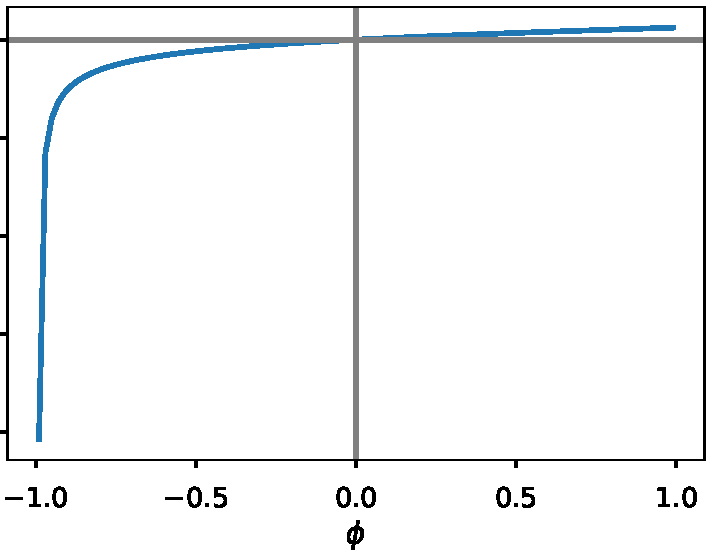
\includegraphics[width=.5\textwidth]{gamma_diff_theta2.pdf}
\end{figure}

\begin{restatable}[Uniform Convergence under Strong Identification]{lemma}{UllnStrongID}
    \label{lemma:UniformConvergenceStrongID}
    Let $\Eta$ be the identified set defined by \cref{eqn:EtaDefn}.
    Further assume that $\phi_0 \neq 0$. 
    Let $\sampmom$ be the sample moment condition defined above, and $\W_T$ be the associated optimal weight matrix
    estimator.
    Then we have the following convergence.

    \begin{align}
        &\sup_{\eta \in \Eta} \norm*{\sampmom(\eta) - \E\left[g\left(\eta \mvert \gamma_0\right)\right]}_{Fro}
          \pto 0 \\ 
        &\sup_{\eta \in \Eta} \norm{\W_{T}(\eta)-\E\left[\W\left(\eta \mvert \gamma_0\right)\right]} \pto 
    \end{align}

\end{restatable}



%TODO where does this go?
By the above arguments, we have a consistent estimator for $\eta$ and the optimal weight matrix $\W \coloneqq
(\E\left[g g'\right])^{-1}$, and we will assume that the true value $\eta_{0}$ is in the interior of its sample
space $\Eta$.\footnote{Throughout we will use subscript \num{0}  to denote true values for parameters.}
Let $G \coloneqq \E\left[\frac{\partial}{\partial \eta} \popmom \right]$
Clearly, $g$ is continuously differentiable, and its derivative $G$ is continuous.
In addition, by the identification discussion $G' W \nabla G$ is nonsingular.


\begin{assump}[Weak Dependence]
    \label{assumption:weak_dependence}
    $z_t \coloneqq \begin{pmatrix} r_{t+1} \\ \sigma^2_{t+1} \end{pmatrix}$ are $\alpha$-mixing with $\alpha_t =
       O\left(T^{-5}\right)$
\end{assump}

Since, $\norm*{g_t}$ is almost surely bounded by $1$ it has all of its moments and $z_t$ being $\alpha$-mixing
implies $g_t$ is as well by the central limit theorem for strongly mixing process 
$\sqrt{T} \sampmom(\eta^{*}) \dto \N\left(0, \E\left[\W\right]^{-1}\right)$ as required. 
Consequently, by \textcite[theorem 3.2]{newey1994large} we have convergence in distribution as well as convergence
in probability.

\begin{theorem}[Inference for $\eta$ under Strong Identification]
    Assume that $\phi_0  \in (-1,1) \setminus 0$, $\rho_0 \in [0,1)$, and $c_0 > 0$. 
    Further assume that the data are ergodic, stationary, and satisfy \cref{assumption:weak_dependence}.
    Then the following convergence in distribution holds.

    \begin{equation}
    \sqrt{T} (\widehat{\eta}_T - \eta_0) \dto \N\left(0, \left(G' \E[\W] G\right)^{-1}\right)
    \end{equation}
\end{theorem}





\section{Weak Identification Setup}

In this section, take the model described in the previous sections and place it in the setup of
\textcite{andrewsGmm2014} so that we ca analyze the effects of possible lack of identification in the model in a
nice clean way.
The goal here is to perform valid inference for $\pi, \theta$ even when $\phi$ might be zero. 


From the discussion above, we can collect the parameters discussed above into a parameter vector of the following
form,i.e.\@ recall the following: $\eta = \lbrace \rho, c, \delta, \phi, \pi, \theta \rbrace$
To write it in the notation of \textcite{andrewsGmm2014}, we partition $\eta$ into three subsets.

\begin{align}
    \phi &\coloneqq \phi  \in (-1, 1) \\ 
    \zeta &\coloneqq \lbrace \rho, c, \delta, \theta \rbrace \in [0,1) \times \R_{++} \times \R_{++} \times
    \R  \\
    \pi &\coloneqq \pi \in \R 
\end{align}

Let $\Eta$ be the set of possible $\eta$, that as defined above.
It is worth noting that the parameter space has a product form, i.e.\@ the values do not affect the valid values
of the other parameters.

In this environment, $\pi$ is not identified when $\phi = 0$.
Both $\phi$ and $\zeta$ are always identified, and $\zeta$ does not affect the identification of $\pi$.

Let $Q_T(\eta)$ be the GMM criterion function, then the GMM estimator $\hat{\eta}_T$ satisfies the following.


\begin{equation}
    \widehat{\eta}_T \in \Eta\ \text{and}\ Q_T(\hat{\eta}_T) = \inf_{\eta \in \Eta} Q_T(\eta) +
    o\left(T^{-1}\right) 
\end{equation}


Now that we have defined the parameters, we can characterize the set of assumptions necessary for valid inference.
We will work through the assumptions described in \textcite{andrewsGmm2014}.
The set of necessary assumptions is relatively complicated because we have to characterize the asymptotic
distribution under several different estimation strengths simultaneously, and the assumptions required to do that
  differ in the various cases. 
In what follows, we will use 

The first assumption specifies the basic identification
problem. It also provides conditions that are used to determine the
probability limit of the GMM estimator, when it exists, under all categories
of drifting sequences of distributions.
Let $\xi$ index the part of the distribution of the data $r_{t+1}, \sigma^2_{t+1}$ that is not determined by the
moment equations.
In general, it is a (likely infinite-dimensional) nuisance parameter that affects the distribution of the data. 


We collect the parameters that we are estimating $\eta$ and the nuisance parameter $\xi$ into one parameter,
$\gamma$ and associated parameter space $\Gamma$.
In the previous discussion we characterized the parameter spaces in a non-compact fashion, let $\Eta^{*}$ be a
compact subset of $\Eta$, where the true parameter values live.
%TODO Does the set of possible nuisance parameters depend upon the estimated parameters in our model?

\begin{defn}{Complete Parameter Space}
    \begin{equation}
        \Gamma \coloneqq \left\lbrace \gamma = (\eta, \xi) \mvert \eta \in \Eta, \xi \in \Xi \right\rbrace 
    \end{equation}
\end{defn}

We characterize these drifting sequences of distributions by sequences of true parameters $\gamma_T \coloneqq
(\eta_T, \phi_T)$.


\begin{restatable}[Inference for $\eta$ under Weak Identification]{theorem}{InferenceWeakID}
    Let that $\phi_0  \in (\underline{\phi}_0,1)$, for some $\underline{\phi}_0 > -1$. 
    $\rho_0 \in [0,1)$, and $c_0 > 0$. 
    Further assume that the data are ergodic, stationary, and satisfy \cref{assumption:weak_dependence}.
    Then the following convergence in distribution holds.

    \purple{TODO Add Conclusion}
\end{restatable}


\clearpage

\phantomsection
\addcontentsline{toc}{section}{References}
\printbibliography
\clearpage

\begin{appendices}

\section{Assumptions}

    In what follows, three sets of drifting sequences $\lbrace \gamma_T \rbrace$ are key. 
    
    \begin{defn}{Drifting Sequence Parameter Spaces}
        \begin{align}
            \Gamma\left(\gamma_0\right) &\coloneqq \left\lbrace \left\lbrace \gamma_T \in \Gamma \right\rbrace
            \mvert \gamma_T \to \gamma_0 \in \Gamma \right\rbrace\\ 
            \Gamma(\gamma_0, 0, b) &\coloneqq \left\lbrace \lbrace \gamma_T \rbrace \in \Gamma(\gamma_0) \mvert
            \phi_0 = 0\ \text{and}\ \sqrt{T} \phi_T \to b \in (\R \cup \lbrace \pm \infty) \right\rbrace \\
            \Gamma(\gamma_0, \infty, b_0) &\coloneqq \left\lbrace \lbrace \gamma_T \rbrace \in \Gamma (\gamma_0)
            \mvert \sqrt{T} \phi_T \to \infty\ \text{and}\ \phi_T \to b_0 \right\rbrace 
        \end{align}
    \end{defn}
    
    These are the standard GMM regularity conditions appropriately adjusted for the lack of identification when $\phi
    =0$.
    
    
    \begin{assump}[GMM 1]\label{ass:GMM1}
    \begin{assumplist}
        \item If $\phi_0=0$, $\sampmom(\eta)$ and $\W_{T}(\eta)$ do not depend on $\pi$ for all $\eta \in \Eta$,
            for all $T \geq 1$, and for all $\gamma^{*}\in \Gamma.$ 
            \label{ass:GMM1a}
        \item If $\lbrace \gamma_{T} \rbrace \in \Gamma\left(\gamma_0\right)$, $\sup_{\eta \in \Eta}
            \norm*{\sampmom(\eta) - \E\left[g\left(\eta \mvert \gamma_0\right)\right]} \pto 0$ and $\sup_{\eta
            \in \Eta} \norm{\W_{T}(\eta)-\E\left[\W\left(\eta \mvert \gamma_0\right)\right]} \pto 0$.
            \label{ass:GMM1b}
        \item When $\phi_0 = 0$,  $g_0\left(\phi, \zeta ,\pi \mvert \gamma_0\right) = 0$ if and only if $\phi
            =\phi_0$ and $\zeta = \zeta_0$ for all $\pi \in \Pi$ and for all $\gamma_0 \in \Gamma.$
            \label{ass:GMM1c}
        \item When $\phi_0 \neq 0$, $g_0\left(\eta \mvert \gamma_0\right)=0$ if and only if $\eta =\eta_0$ for all
            $\gamma_0 \in \Gamma.$
            \label{ass:GMM1d}
        \item  $g_0\left(\eta \mvert \gamma_0\right)$ is continuously differentiable in $\eta $ on $\Eta$ with
            partial derivatives with respect to $\eta$ and $\xi$ denoted by $g_{\eta}\left(\theta \mvert
            \gamma_0\right) \in R^{k\times d_{\eta }}$ and $g_{\xi }\left(\eta \mvert \gamma_0\right)\in R^{k\times
            d_{\xi }}$, respectively.
            \label{ass:GMM1e}
        \item $\W\left(\eta \mvert \gamma_0\right)$ is continuous in $\eta$ on $\Eta$ for all $\gamma_0\in
            \Gamma$.  \label{ass:GMM1f}
        \item $0 < \lambda_{\min}(\W\left(\xi_0, \pi \mvert \gamma_0\right))\leq \lambda_{\max }(\W\left(\xi_0,\pi
            \mvert \gamma_0\right)) < \infty$, $\forall \pi \in \Pi$, for all $\gamma_0 \in \Gamma$.
            \label{ass:GMM1g}
        \item $\lambda_{\min} (g_{\xi}\left(\xi_0,\pi \mvert \gamma_0\right)^{\prime} \W\left(\xi_0,\pi \mvert
            \gamma_0\right)g_{\xi }\left(\xi_0,\pi \mvert \gamma_0\right))>0$, for all $\pi \in \Pi$,  and for all 
            $\gamma_0 \in \Gamma$ with $\phi_0=0.$
            \label{ass:GMM1h}
        \item$\Xi(\pi)$ is compact for all $\pi \in \Pi$, and both $\Pi$ and $\Eta$ are compact.
            \label{ass:GMM1i}
        \item For all $\epsilon > 0$, there exits a $\delta > 0$ such that $d_{H}\left(\Xi \left(\pi_{1}\right),
            \Xi \left( \pi_{2}\right) \right) < \epsilon$ for $\pi_{1}, \pi_{2} \in \Pi$ with
            $\norm*{\pi_{1}-\pi_{2}} < \delta$, where $d_{H}\left( \cdot \right)$ is the Hausdorff metric.
            \label{ass:GMM1j}
    \end{assumplist}
    \end{assump}
    
    
    
    \begin{assump}[GMM 2*]\label{ass:GMM2}
    \begin{assumplist}
        \item $\sampmom(\eta)$ is continuously differentiable in $\eta$ for all $T \geq 1$. 
            \label{ass:GMM2a}
        \item If $\{\gamma_T\} \in \Gamma\left(\gamma_0, 0, b\right)$, $\sup_{\left\lbrace \eta \in \Eta \mvert
            \norm*{(\phi, \zeta')' - (\phi_T, \zeta_0')} \leq \delta_T \right\rbrace}
            \norm*{\frac{\partial}{\partial (\phi, \zeta')'} \sampmom(\eta) - \E\left[\popmom_{(\phi,
            \zeta')'}(\eta) \mvert \gamma_0\right]} = o_p(1)$ for all deterministic sequences  $\delta_T \to 0$.
            \label{ass:GMM2b}
        \item[] \purple{(Xu) : Is this a valid translation of the relevant domain?}
        \item If $\{\gamma_T \} \in \Gamma\left(\gamma_0, \infty, b_0\right)$, $\sup_{\left\lbrace \eta \in
            \Eta \mvert \norm*{\eta - \eta_0} \leq \delta_T \right\rbrace} \norm*{\left(\frac{\partial}{\partial
            \eta'} \overline{g}_T - \E\left[g_{\eta}(\eta) \mvert \gamma_0\right]\right)
            \diag\left(1_{1+d_\zeta}', (1/\phi_T)_{d_{\pi}}'\right)}  = o_p(1)$ for all deterministic sequences
            $\delta_T \to 0$.
            \label{ass:GMM2c}
    \end{assumplist}
    \end{assump}
    
    Once we have \nameref{ass:GMM1} and \nameref{ass:GMM2}, we use \nameref{ass:GMM3} to derive the asymptotic
    distribution under weak and semi-strong identification.
    These conditions will be characterized using the expected derivative of the population moment conditions. 
    
    \begin{defn}
        \label{defn:moment_derivative_func}
        \begin{equation}
            K_{T,g}\left(\eta \mvert \gamma^{*}\right) \coloneqq  \frac{1}{T} \sum_{i=1}^T \frac{\partial}{\partial
            \phi^{*}} \E \left[ \popmom(W_T, \eta) \mvert \gamma^{*} \right]
        \end{equation}
    \end{defn}
    
    
    \begin{assump}[GMM 3]\label{ass:GMM3}
    \begin{assumplist}
        \item $\sampmom(\eta) = \frac{1}{T} \sum_{i=1}^T \popmom(W_T, \eta)$  for some function $\popmom(W_T,
            \eta) : \R^{k \times k} \times \Eta \to \R^k$.
            \label{ass:GMM3a}
        \item $\E\left[\popmom(W_T, \beta_0, \zeta^{*}, \pi) \mvert \gamma^{*} \right] = 0$ for all $\pi \in \Pi$ and
            for all $i \geq 1$ if $\gamma^{*} = \left(0,\zeta^{*}, \pi^{*}, \xi^{*} \right) \in \Gamma$.
            \label{ass:GMM3b}
        \item If $\{ \gamma_T \} \in \Gamma(\gamma_0, 0, b)$, $\frac{1}{\sqrt{T}} \sum_{i=1}^T \left(g(W_T,
            \zeta_{0,T}, \pi_T) - \E \left[g(W_T, \zeta_{0,T}, \pi_T)\mvert \gamma_T \right]\right)  \dto \N\left(0,
            \aleph(\gamma_0)\right)$, where $\aleph(\gamma_0)$ is a $k \times k$ matrix.
            \label{ass:GMM3c}
        \item 
            \label{ass:GMM3d}
            \begin{enumerate}
                \item  $K_{T,g}\left(\eta \mvert \gamma^{*}\right)$ exists for all $\{\eta, \gamma^{*} \} \in
                    \left(\Eta_{\delta} \times \Gamma_{0}\right)$ and for all $T \geq 1$.
                \item $K_{T,g}\left(\phi_T, \zeta_T, \pi \mvert \widetilde{\gamma}_T\right)$ uniformly converges
                    to some non-stochastic matrix-valued function  $K_{g}\left(0, \zeta_0, \pi \mvert
                    \gamma_0\right)$ over $\pi \in \Pi$ for all deterministic sequences $\{\phi_T, \zeta_T,
                    \widetilde{\gamma}_T \}$ satisfying $\widetilde{\gamma}_T \in \Gamma$, $\widetilde{\gamma}_T
                    \to \gamma_0 \coloneqq (0, \zeta_0, \pi_0, \xi)$, $\{\phi_T, \zeta_T, \pi \} \in \Eta$ and
                    $\{\phi_T, \zeta_T \} \to (0, \zeta_0)$.
                \item $K_g\left(\phi_0, \zeta_0, \pi \mvert \gamma_0\right)$ is continuous on $\Pi$ for all
                    $\gamma_0 \in \Gamma$ with $\phi_0 = 0$.
            \end{enumerate}
            \item $K\left(\phi_0, \zeta_0, \pi \mvert \gamma_0\right) = \popmom_{\phi, \zeta}\left(\phi_0,
                \pi\mvert \gamma_0\right) x$ for some $x \in \R^{1+d_{\zeta}}$ if and only $\pi =
                \pi_0$.\footnote{Since $\dim(\phi) = 1$, we can assume without loss of generality that the
                $\omega_0$ from \textcite{andrewsGmm2014} equals $1$.}
                \label{ass:GMM3e}
            \item If $\{ \gamma_T \} \in \Gamma(\gamma_0, 0, b)$, $\frac{1}{T} \sum_{i=1}^T
                \frac{\partial}{\partial \eta}  \E\left[ \popmom\left(W_T, \eta_T \right ) \mvert \gamma_T \right]
                \to \popmom_{\eta}\left(\eta_0 \mvert \gamma_0\right)$.
            \label{ass:GMM3f}
    \end{assumplist}
    \end{assump}

    \begin{defn}{\popmom*}
        \begin{equation}
            g_{\phi, \zeta}^{*}\left(\phi_0, \zeta_0, \pi_1, \pi_2 \mvert \gamma_0\right)  =
            \left[g_{\phi}\left(\phi_0, \zeta_0, \pi_1 \mvert \gamma_0\right)  , g_{\phi}\left(\phi_0, \zeta_0,
            \pi_2 \mvert \gamma_0\right) , g_{\zeta} \left(\phi_0, \zeta_0 \mvert \gamma_0\right)  \right]  \in
            \R^{k \times (d_{\zeta} + 2)}
        \end{equation}
    \end{defn}


    \begin{assump}[GMM 4]\label{ass:GMM4}
    \begin{assumplist}
        \item $\phi$ is a scalar.
        \item $g_{\phi, \zeta}^{*}\left(\phi_0, \zeta_0, \pi_1, \pi_2 \mvert \gamma_0\right)$ has full column
            rank. 
        \item $\aleph(\gamma_0)$ is positive definite for all $\gamma_0 \in \gamma $ with $\phi_0 = 0$. 
    \end{assumplist}
    \end{assump}

    \section{Proofs}

    \identifiedSet*

    \begin{proof}
    
    Since the exponential function is a strictly positive function, and we are considering a grid of $x$ values, a
    sufficient condition for $\rho, \delta$, \& $c$ to be identified is for the relevant rows of $\nabla a(x)$ and
    $\nabla b(x)$ to equal zero only at $\eta_{0}$ which are satisfied if $\rho, c, \delta > 0$.
    Testing if if $\phi$ and $\theta$ are identified is somewhat trickier. 
    Consider $\nabla \alpha(x)$. 
    Since we are using a grid of $x$'s, and the gradient of $\alpha$ is a nonlinear function of $x$, the first two
    rows of the \cref{eqn:alpha_gradient} imply $\phi$ is identified.
    
    \begin{equation}
        \label{eqn:alpha_gradient}
        \frac{\partial \alpha(x)}{\partial (\phi, \theta, c)'}  = \begin{bmatrix} \phi x^{2} + x \left(- 2 \beta
        \left(\theta_{2} - \frac{1}{2}\right) - \frac{\phi}{2 \sqrt{c} \left(\phi + 1\right)^{\frac{3}{2}}} +
        \frac{1}{\sqrt{c} \sqrt{\phi + 1}}\right) \\ x \left(- \phi^{2} + 1\right) \\ \frac{\phi x}{2
        c^{\frac{3}{2}} \sqrt{\phi + 1}} \end{bmatrix} 
    \end{equation}
    
    The top line of \cref{eqn:alpha_gradient} can be solved for $\theta$, which would create a local lack of
    identification for $\theta$.
    However, this creates a linear relationship between $\theta$ and the other parameters and $x$.
    However, since we are using multiple $x$'s we can avoid this issue.
    Consequently,  $\phi \in (-1,1], c > 0$, are sufficient to identify all of the parameters except for $\pi$,
    the price of volatility risk.
    We can use \cref{eqn:a(x)} to identify $\rho$.
    
    If $\phi = 0$, $\beta(x) = x \left(a (\pi + \alpha(\theta)) - a(\pi + \alpha(\theta))\right)$, and
    $\gamma(x) =  x \left(b (\pi + \alpha(\theta)) - b(\pi + \alpha(\theta))\right)$.
    These both  identically zero, and $\pi$ does not show up in anywhere  else in the criterion function.
    
    \end{proof}


\UllnStrongID*

\begin{proof}

    In this proof we rely heavily on the continuity of the moment conditions over their domain. 
    This can be seen from simple inspection since we assumed that $\phi_0 \geq \underline{\phi} -1$.
    Furthermore since $\Eta$ is compact, this continuity implies uniform continuity.
    
    For any positive definite weight-matrix by \textcite[Lemma 2.3]{newey1994large} our criterion function has
    a unique optimum.
    The data, $\sigma^2_{t+1}, r_{t+1}$, are ergodic and stationary.
    Since the moment conditions are not redundant the optimal (GMM) weight matrix $\W$ is positive definite. 
    In addition, $\popmom$ is continuous at each $\eta$, given the restrictions above and properties of
    characteristic functions imply that $\popmom$ is uniformly bounded. 
    For convenience, we assume that the space of $\eta$ is compact.
    This should not be an issue here because the parameters  are either a priori bounded, such as $\phi$ or we
    have substantial a priori knowledge on their plausible magnitudes.
    Hence, \textcite[Theroem 2.6]{newey1994large} implies our estimator is consistent.
    
    However, when we allow for weak identification late on, we need this convergence to be uniform. 
    One straightforward way to show this is to show that our criterion function is globally Lipschitz in a set of
    high probability. 
    
    The other issue is that we need the weight matrix to converge uniformly to its expectation.
    Since the moments are continuous functions over their domain as is the square function.
    This convergence is uniform if and only if the matrix inverse is continuous.
    
    Since we have a finite number of non-redundant moments, the minimum eigenvalue, \\
    $\lambda_{min}\left(\W\left(\phi_0, \zeta_0, \pi \mvert \gamma_0\right)\right) > 0$, and so the matrix inverse
    is uniformly continuous in $\gamma_0$ with respect to the Frobenius norm, which is the sum of the eigenvalues.
    (Recall, that the eigenvalues of the inverse are the inverse of the eigenvalues.)


\end{proof}

\InferenceWeakID*

\begin{proof}
We prove this result by showing that Assumptions GMM 1-4 are satisfied.

\begin{proofpart}
    \label{part:main_theorem_proof_part1}
    In this part, we show that \nameref{ass:GMM1} is satisfied. 
    To do this, we break \nameref{ass:GMM1}  down into three subsections.
    Assumptions \namedref{ass:GMM1a}, \namedref{ass:GMM1b}, \namedref{ass:GMM1c}, and \namedref{ass:GMM1d} state
    that when $\phi = 0$, the moment conditions contain no information regarding $\pi$, but when $\phi \neq 0$,
    the model is identified.
    This is what we show in \cref{lemma:IdentifiedSet}.
    We further showed the relevant uniform convergence to verity \namedref{ass:GMM1b} in
    \cref{lemma:UniformConvergenceStrongID}.
    
    The next two assumptions (\namedref{ass:GMM1e} and \namedref{ass:GMM1f} are  technical conditions regarding the
    behavior of the moment conditions and weight matrix. 
    Since our moment conditions are derived from an infinitely-differentiable  characteristic function and the
    weight matrix is the optimal one, they both hold trivially.
    
    The third subsection of Assumption \nameref{ass:GMM1} concerns the weight matrix.
    Since we are using the inverse covariance matrix of valid non-redundant model, assumptions
    \namedref{ass:GMM1g} and \namedref{ass:GMM1h} automatically hold.
    
    The last two assumptions, \namedref{ass:GMM1i} and \namedref{ass:GMM1j} require that the parameter spaces do
    not vary too much with the parameters and are compact.
    Since $\Eta$ is compact, \namedref{ass:GMM1i} holds trivially, and since it has  has a product form,
    \namedref{ass:GMM1j}  holds trivially as well.
    
\end{proofpart}


\begin{proofpart}
    In this section, we show that the derivatives of the moment conditions have the correct behavior locally to
    the true parameters.
    We have to do this for the different classes of drifting sequences.

    Since our moment conditions are sample averages of the characteristic function, they satisfy
    \namedref{ass:GMM2a} automatically. 

    \purple{TODO: We need to show that \namedref{ass:GMM2b} and \namedref{ass:GMM2c} are satisfied (they are)
    using a uniform law of large numbers and the dominated convergence theorem.}
    \textcite{andrewsGmm2014} show that this is a sufficient condition for their Assumption GMM2, which is what we
    actually need. 

    Since characteristic functions are uniformly bounded, by the dominated convergence theorem we can interchange the 
    expectation and derivative operators. 
    Hence \namedref{ass:GMM3b} and \namedref{ass:GMM3c} are equivalent to the statements in terms of the moment
    conditions them selves mutatis mutandis.  
    In addition, sice the derivate is a linear operator, we can pull it outside of the norm.
    The reason that the uniform law of large numbers in \cref{part:main_theorem_proof_part1} does not trivially
    imply this result is because we are not considering sequences $\phi_T \to \phi_0$. 

    We start by showing \namedref{ass:GMM2b}. 
    Assume that $\lbrace \gamma_T \rbrace \in \Gamma\left(\gamma_0, 0, b\right)$.
    We know by \cref{lemma:IdentifiedSet} that if $\phi_0=0$, the moment condition is independent of $\pi$. 

    %should I use a mean value expansion?
    We create a mean value expansions around around $(\phi_0, \zeta_T, \pi_T$ of the sample moment condition and
    around $\phi_0, \zeta_0, \pi_0$ for the population moment condition.
    (This is not the same in both cases, not is it the true parameter for the drifting sequence in the case of the
    sample moment condition.)
    In addition, also since we are considering continuous functions of compact spaces, The $\delta_T$ ball in
    $\R^{\dim(\eta)}$, convergence implies uniform convergence, and so we only need to show convergence below.


    \begin{alignat}{2}
        & &&\norm*{\sampmom(\phi_T, \zeta_T, \pi_T) -  \popmom(\phi_0, \zeta_0, \pi_0)} \\ 
        \intertext{We take a mean value expansion of both functions. The point at which the derivative in the two
        locations is taken may not be the same.}
        &= &&\left\lVert \sampmom(\phi_0, \zeta_T, \pi_T) + \frac{\partial}{\partial (\phi, \zeta,
           \pi)}\sampmom(\widetilde{\phi}, \widetilde{\zeta}, \widetilde{\pi})(\phi_0, \zeta_0, \pi_0) \right. \\
        &  &&\quad \left. - \E\left[\popmom(\phi_0, \zeta_T, \pi_0) \mvert \gamma_0\right] +
           + \frac{\partial}{\partial (\phi, \zeta, \pi)} \E\left[\popmom(\widetilde{\phi}, \widetilde{\zeta},
           \widetilde{\pi})\mvert \gamma_0\right] (\phi_0, \zeta_0, \pi_0)  \right\rVert \\ 
    \end{alignat}


\end{proofpart}

Assumption \namedref{ass:GMM3a} is trivially satisfied,  and we showed that \namedref{ass:GMM3b} is satisfied in
\cref{sec:spectral_GMM}.
    \purple{TODO: Show that \nameref{ass:GMM3c} is sasfied by using a triangular CLT}



First, start by defining $g^{*}$ as follows, where (as used above) $g_{x}$ refers to the derivative of $g$ with
respect to $x$.
Note, assumptions \namedref{ass:GMM1a} and \namedref{ass:GMM3a}  imply that when $\phi_0 = 0$,
$g_{\zeta}\left(\phi_0, \zeta_0, \pi \mvert \gamma_0\right)$, does not depend upon $\pi$.

\end{proof}


\end{appendices}


\end{document}


